\section{Printplade}
\subsection{Design af printplade}
\vspace{0.5 cm}
For at kunne designe et printudlæg skal kredsløbet realiseres i Multisim. Kredsløbet opbygges derfor med de beregnede komponentværdier til henholdsvis forstærker, subtractor og filter. \\
Når kredsløbet er realiseret i multisim kan diagrammet overføres til Ultiboard hvor printpladen kan opstilles med korrekte forbindelser mellem komponenterne.
\subsubsection{Multisim}
\begin{figure}[h!]
	\centering
	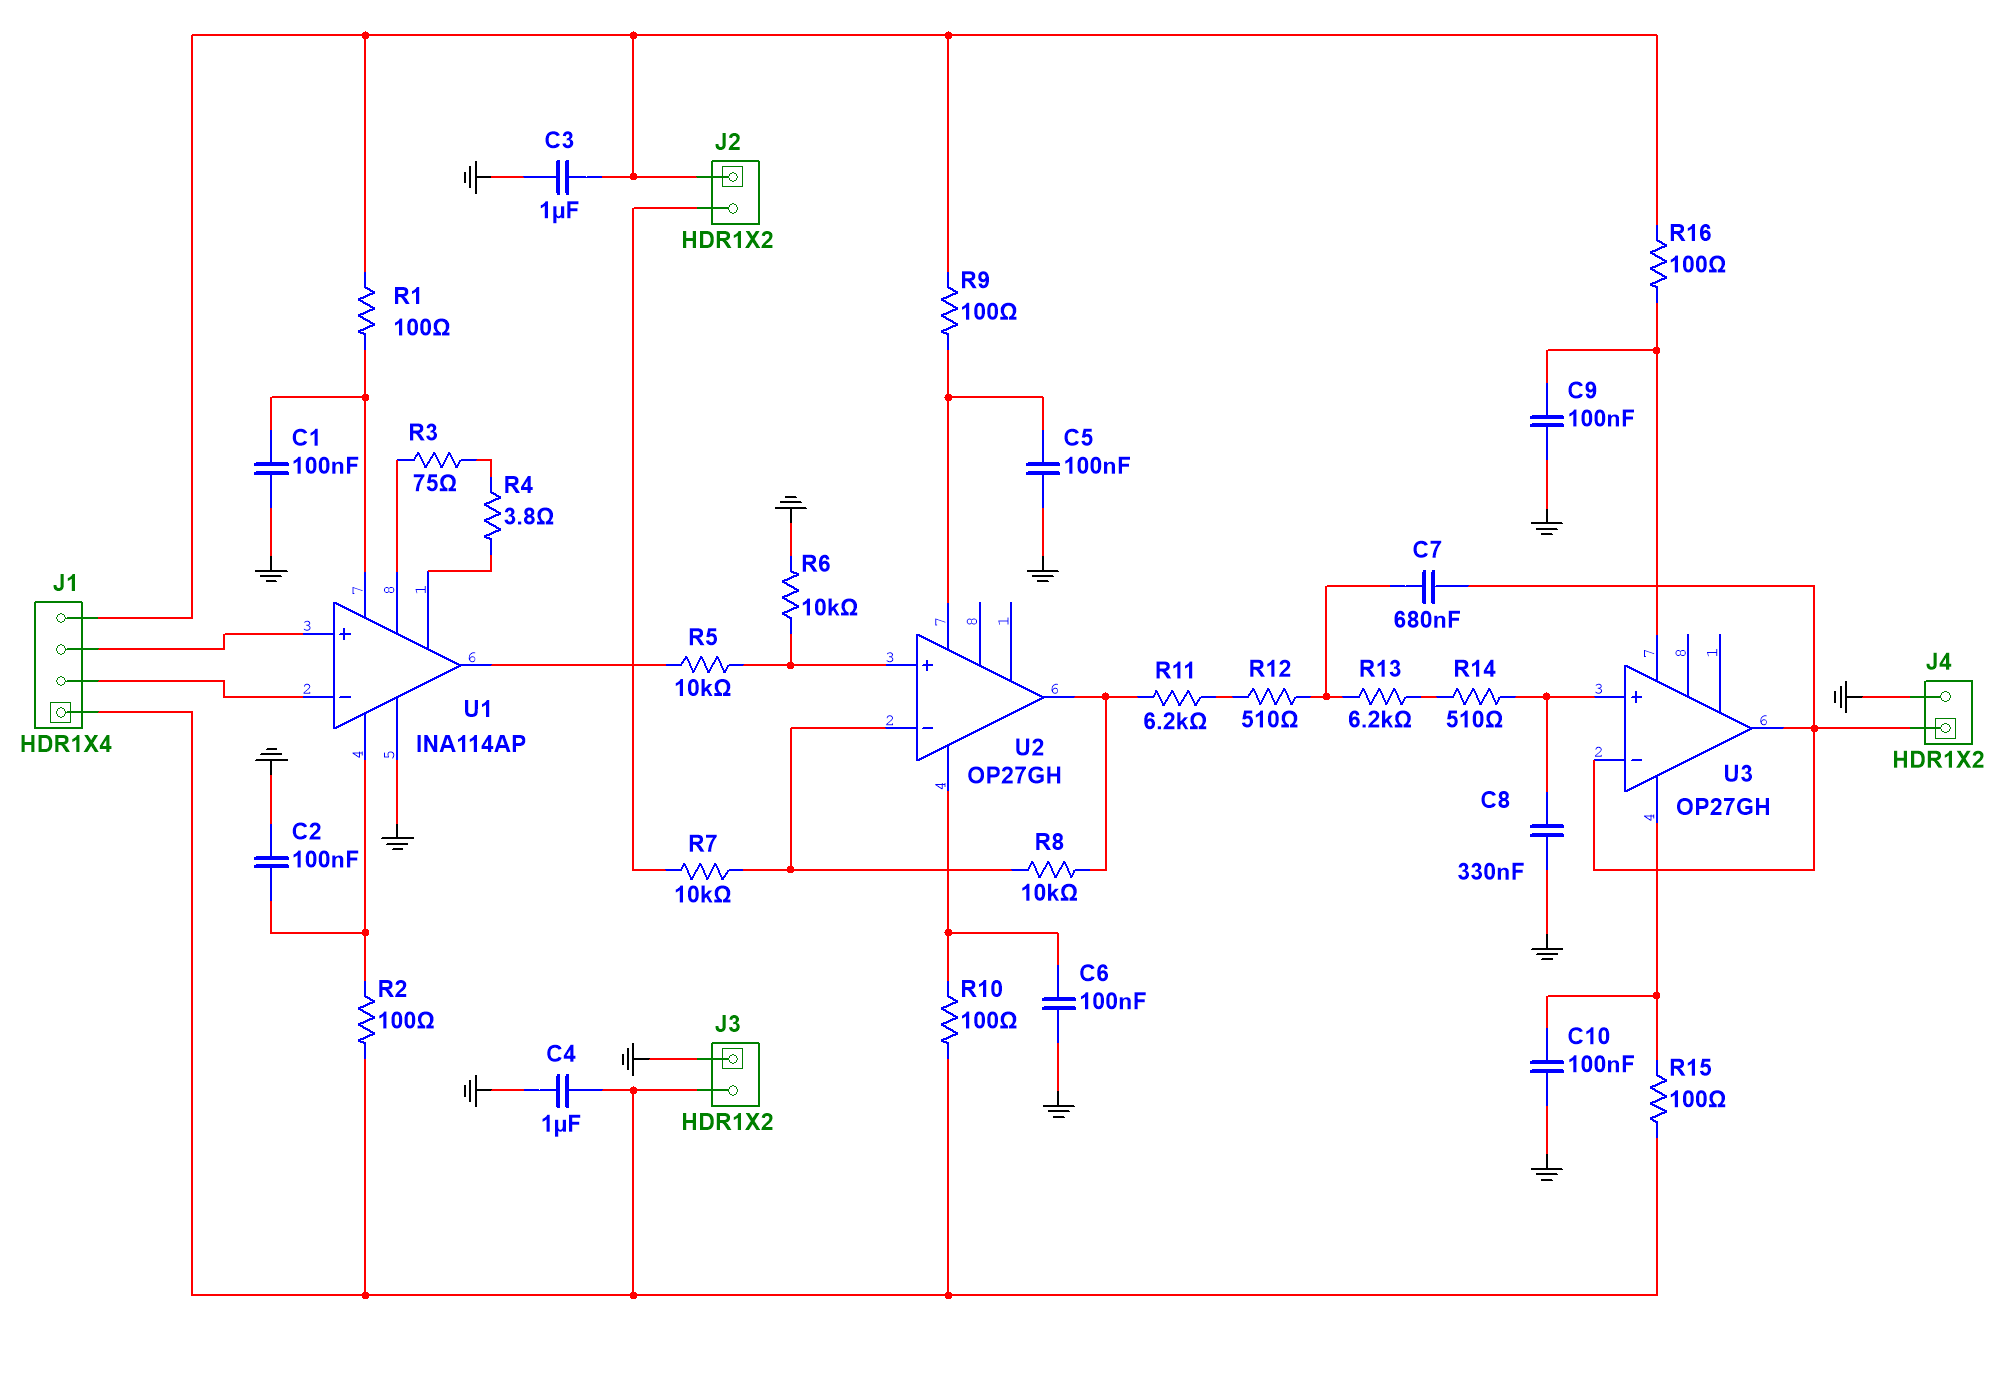
\includegraphics[width=1\linewidth]{Hardware/Multisim}
	\caption{Kredsløbets opbygning i Multisim}
	\label{fig:Multisim}
\end{figure}

På figur \vref{fig:Multisim} ses kredsløbet opbygget med korrekte komponentværdier. Til venstre i diagrammet ses en header J1, der på den designede printplade skal udgøre de fire forbindelser til tryktransduceren. Øverst ses en header J2, der skal udgøre strømforsyningen - henholdsvis 5V til transducer, forstærker og filter samt en 2V strømforsyning til substractoren. Nederst i diagrammet ses en header J3, der skal udgøre -5V og stelforbindelse. Til højre i diagrammet ses en header J4, der skal bruges til at forbinde printpladen til AD-Converteren.

\vspace{0.3 cm}

For at sikre systemet mest muligt mod støj stabiliseres signalet med afkoblingskondensatorer. De ses henholdsvis på strømforsyning, 5V og -5V samt på forstærker, subtractor og filter. Afkoblingskondensatorer er placeret så tæt på som muligt. 

\clearpage

\subsubsection{Ultiboard}
\vspace{0.5 cm}
\begin{figure}[h!]
	\centering
	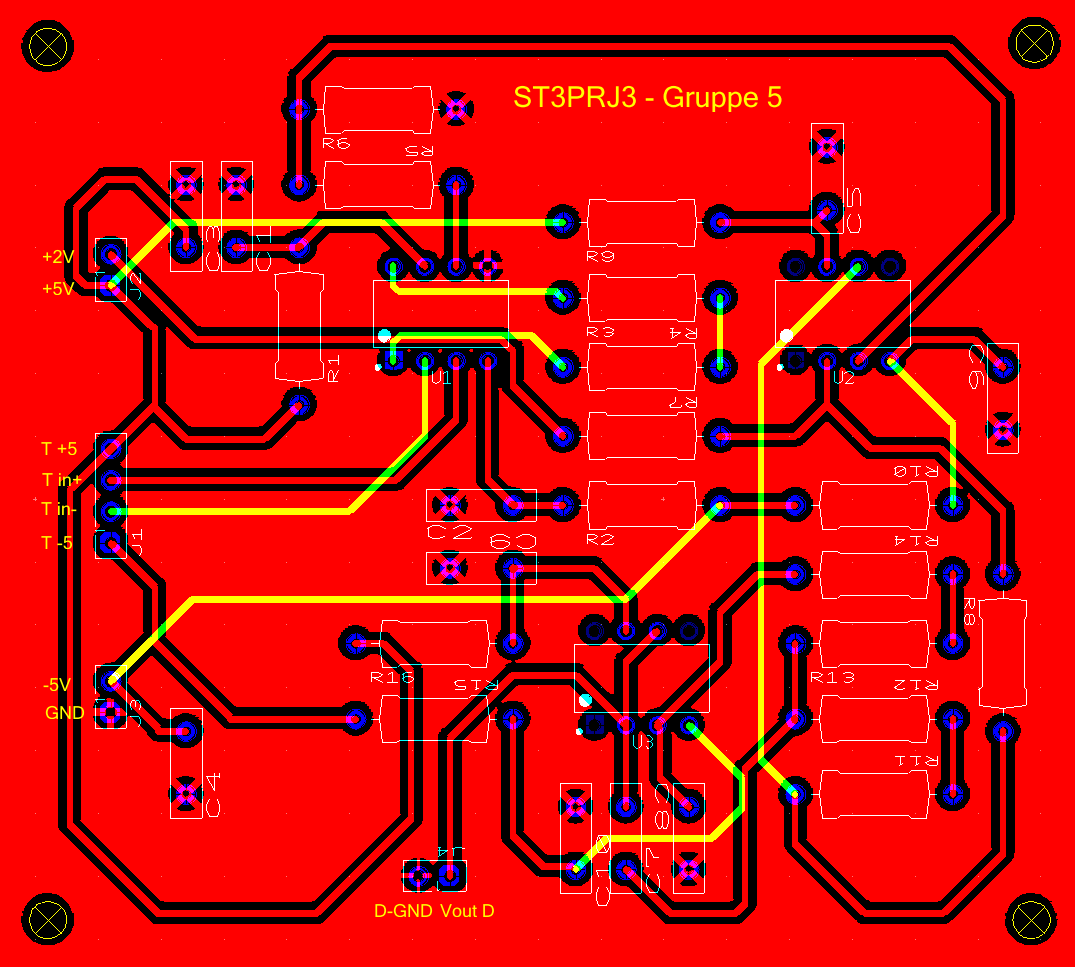
\includegraphics[width=0.6\linewidth]{Hardware/Ultiboard}
	\caption{Design af printplade i Ultiboard}
	\label{fig:Ultiboard}
\end{figure}

\vspace{0.5 cm}

På \vref{fig:Ultiboard} ses kredsløbet fra Multisim overført til Ultiboard. Forstærker og subtractor er placeret øverst på pladen hvorimod filteret er placeret nederst på pladen. Mocstande og kondensatorer er placeret så tæt som muligt for at gøre det mere organiseret og overskueligt at kigge på. Strømforsyning, stelforbindelse og indgang til transducer er placeret til venstre på pladen. Udgangen til AD-Converteren ses nedest på pladen.

\clearpage
\subsection{Test af printplade}
\vspace{0.5 cm}
\subsubsection{Multisim}
Til at teste kredsløbet for eventuelle fejl i opbygningen realiseres diagrammet i Multisim. 

INDSÆT TEKST OG BILLEDE HÉR

\subsubsection{Ultiboard}
For at være sikker på, at printpladen er opbygget i Ultiboard uden fejl kan der udføres forskellige tests inde i programmet. Det tjekkes visuelt, at at forbindelser mellem komponenterne er lavet og der derfor ikke er nogle overskydende ratsnest tilbage. Disse ratsnests er de gule linjer, der viser forbindelserne mellem komponenterne før forbindelserne er tegnet.

\begin{figure}[h!]
	\centering
	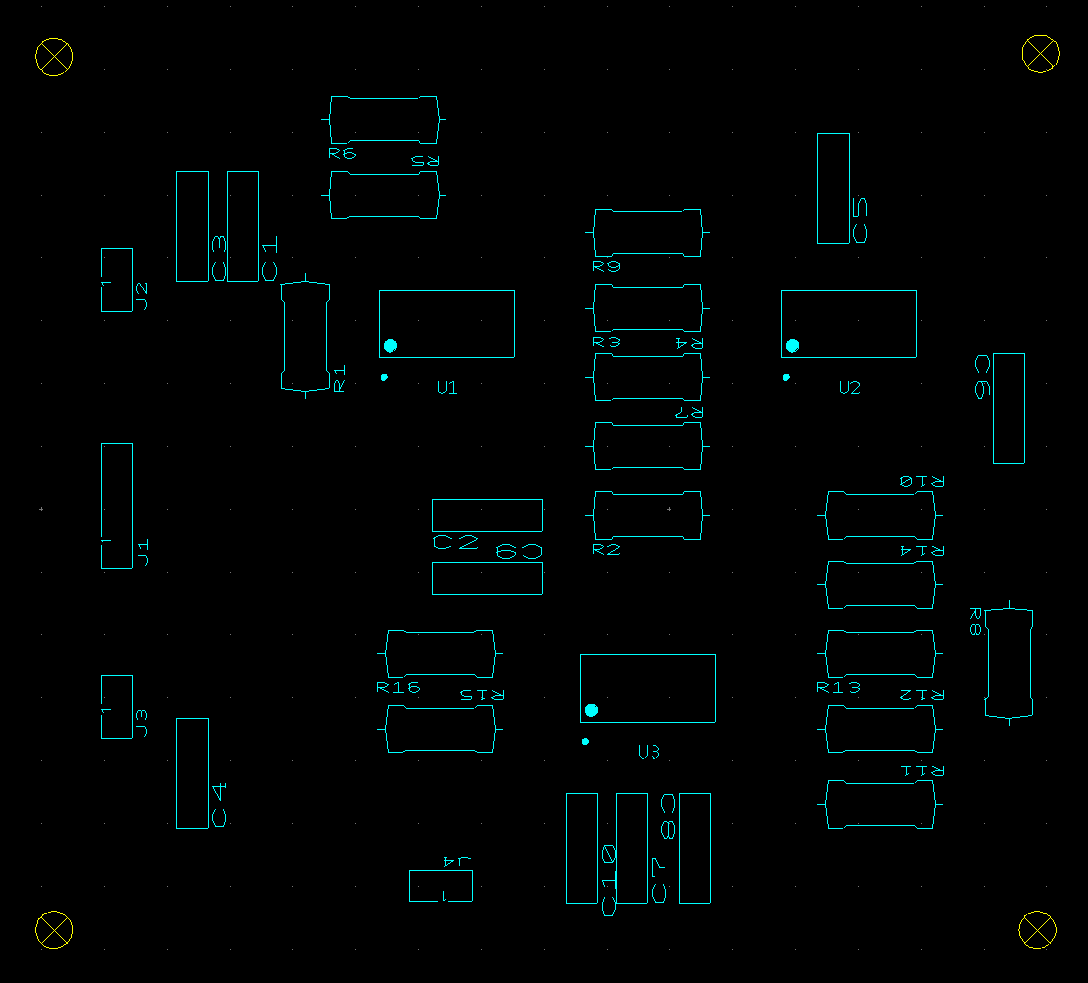
\includegraphics[width=0.6\linewidth]{Hardware/Ratsnest}
	\caption{Test af printplade: Ratsnests}
	\label{fig:Ratsnest}
\end{figure}

Ud over at teste for manglende forbindelser mellem komponenter kan man lave lignende tests, der henholdsvis tester nets for fejl og mangler samt en overordnet test, der tester for fejl. Disse tests ses på figurerne nedenfor. 

\begin{figure}[h!]
	\centering
	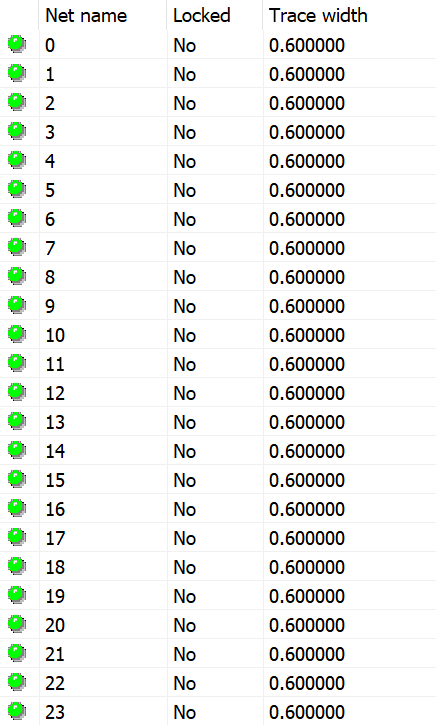
\includegraphics[width=0.2\linewidth]{Hardware/Nets}
	\caption{Test af printplade: Nets}
	\label{fig:Nets}
\end{figure}

\begin{figure}[h!]
	\centering
	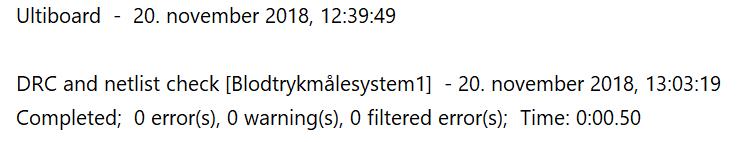
\includegraphics[width=0.6\linewidth]{Hardware/Fejl}
	\caption{Test af printplade: Fejl}
	\label{fig:Fejl}
\end{figure}

\subsection{EuroCircuits}
Før printpladen bestilles laves en sidste test, der tester for, om printpladen kan laves. Denne test er udført på EuroCircuits hjemmeside.

\begin{figure}[h!]
	\centering
	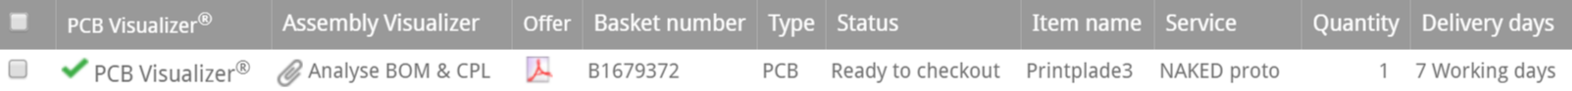
\includegraphics[width=0.8\linewidth]{Hardware/EuroCircuits1}
	\caption{Test af printplade: Nets}
	\label{fig:EuroCircuits1}
\end{figure}

\begin{figure}[h!]
	\centering
	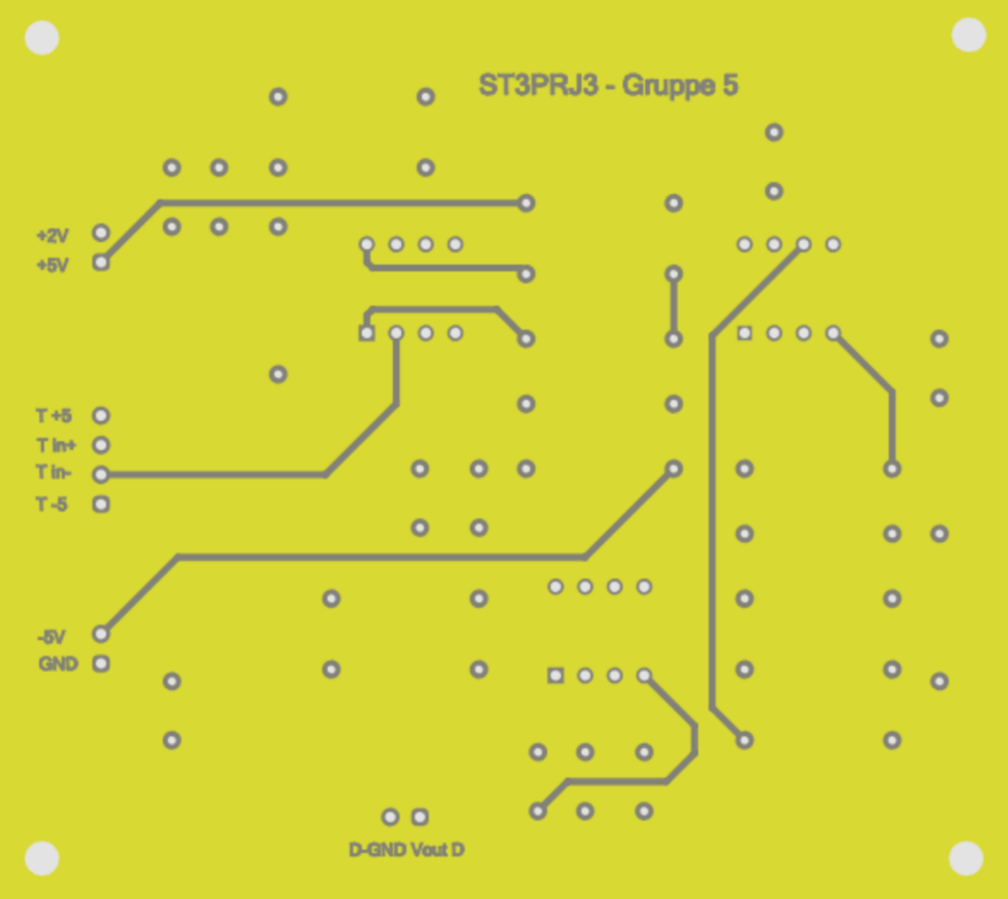
\includegraphics[width=0.5\linewidth]{Hardware/EuroCircuits2}
	\caption{Test af printplade: Fejl}
	\label{fig:EuroCircuits2}
\end{figure}
 
